\documentclass[11pt]{article}

\usepackage[a4paper,margin=1in]{geometry}
\usepackage{amsmath,amssymb,amsthm}
\usepackage{graphicx}
\usepackage{microtype}
\usepackage[hidelinks]{hyperref}

\newtheorem{proposition}{Proposition}
\newcommand{\F}{\mathrm F}

\title{The Fitzpatrick Extension Need Not Be Quasidense\\
A Later-Literature Resolution of arXiv:1612.02500}
\author{Run \texttt{fa\_banach\_001}, lane 7}
\date{12 August 2026}

\begin{document}
\maketitle

\begin{center}
\fbox{\parbox{0.91\textwidth}{\textbf{Status.}
Already answered in the literature.  Simons's later arXiv:2407.00479 gives
an explicit negative answer, so this target is not a new-result candidate.}}
\end{center}

\section{Source question}

Let $S:E\rightrightarrows E^*$ be closed, monotone, and quasidense.  The
source paper proves that its Fitzpatrick extension
$S^\F:E^*\rightrightarrows E^{**}$ is maximally monotone, then asks whether
$S^\F$ must itself be quasidense \cite[Remark~3.10, p.~9]{source}.

\begin{figure}[ht]
  \centering
  
\includegraphics[width=\textwidth]{figures/source_question_crop.png}
  \caption{The question in arXiv:1612.02500v4, PDF page 9.}
\end{figure}

\section{Explicit later answer}

The 2024 paper \emph{Faces of quasidensity} uses $M^\sharp$ for the Gossez
extension of a maximally monotone set $M\subset E\times E^*$.  For
$M=G(S)$ this is exactly the graph of the source paper's Fitzpatrick
extension: both consist of the pairs $(y^*,y^{**})$ monotonically related to
the canonical image of $G(S)$.  For maximally monotone sets, quasidensity is
equivalent to type (NI) \cite[Theorem~11.1]{answer}.

Define
\[
 U:\ell_1\longrightarrow c_0,\qquad
 (Ux)_n=\sum_{k\ge n}x_k,
\]
and let $S=U^{-1}:c_0\rightrightarrows\ell_1$, so
\[
 G(S)=\{(Ux,x):x\in\ell_1\}.
\]
Also define the tail operator
\[
 T:\ell_1\longrightarrow\ell_\infty,\qquad
 (Tx)_n=\sum_{k\ge n}x_k.
\]

\begin{proposition}
The multifunction $S$ is closed, monotone, and quasidense, but its
Fitzpatrick extension $S^\F$ is not quasidense.
\end{proposition}

\begin{proof}
Simons proves that $G(S)=U^{-1}$ is maximally monotone of type (NI), hence
quasidense, and that
\[
 G(S^\F)=G(S)^\sharp=G(T).
\]
He separately proves that $T$ is maximally monotone but not of type (NI)
\cite[Examples~9.3 and 9.8]{answer}.  Since type (NI) and quasidensity are
equivalent here, $S^\F=T$ is not quasidense.  This is the requested negative
answer.
\end{proof}

\begin{figure}[ht]
  \centering
  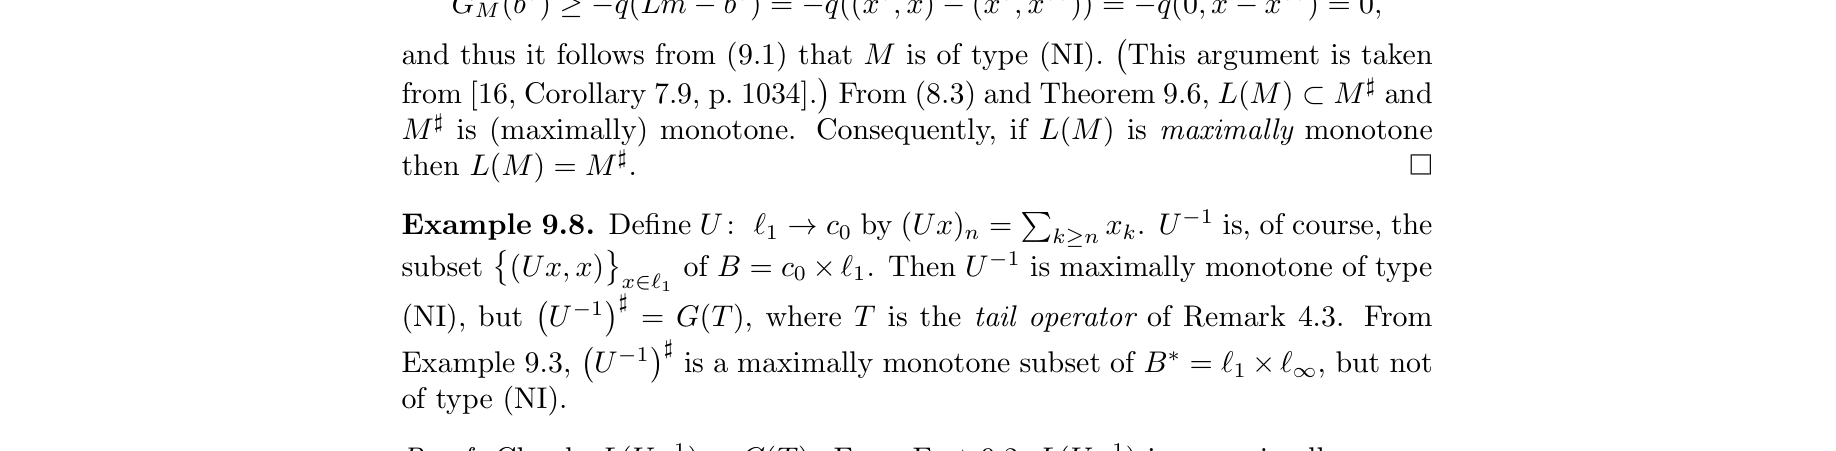
\includegraphics[width=\textwidth]{figures/later_answer_crop.png}
  \caption{The explicit counterexample in arXiv:2407.00479, PDF page 13.}
\end{figure}

For completeness, the later paper certifies failure of type (NI) directly.
Taking $y^*=(1,1,\ldots)\in\ell_\infty$ and a Banach limit
$y^{**}\in\ell_\infty^*$, it obtains, for every $x\in\ell_1$ and
$\sigma=\sum_nx_n$,
\[
 \langle Tx-y^*,\widehat x-y^{**}\rangle
 \ge \tfrac12\sigma^2-\sigma+1
 =\tfrac12(\sigma-1)^2+\tfrac12\ge\tfrac12.
\]
Thus the negative-infimum condition fails by a strict margin.

\section{Assessment}

This is an exact, later primary-source answer to a concrete question in the
target paper.  It is not merely a related result: the later paper explicitly
states that the construction gives a negative answer to the earlier problem,
and its $M^\sharp$ is the same graph as the source's $S^\F$.  Accordingly,
the target should be archived as literature-already-answered rather than
promoted as a new proof or counterexample.

The other broad remarks in arXiv:1612.02500---whether all maximally monotone
operators are type (FPV)/strongly maximal and whether certain proofs can
avoid the bidual---are distinct, long-standing programmatic questions and
are not claimed resolved here.

\begin{thebibliography}{9}
\bibitem{source}
Stephen Simons,
\emph{Quasidense monotone multifunctions},
arXiv:1612.02500v4, 2018.
\url{https://arxiv.org/abs/1612.02500}.

\bibitem{answer}
Stephen Simons,
\emph{Faces of quasidensity},
arXiv:2407.00479, 2024.
\url{https://arxiv.org/abs/2407.00479}.
\end{thebibliography}

\end{document}
